\documentclass[ex,minted]{exercise}

\deadline{21.11.2023}

\begin{document}

\section{Beugung am Einzelspalt}
Das Licht von einem Diodenlaser mit einer Wellenlänge von $445 \u{nm}$ trifft auf einen vertikalen Spalt mit einer Breite
$b = 10 \u{μm}$. In einem Abstand von $L = 20 \u{cm}$ befindet sich hinter dem Spalt ein Schirm.

\subsection{Wie weit sind die Minima der ersten Ordnung auf dem Schirm auseinander?}
\begin{align*}
    \sin\alpha_n &= n \frac\lambda b\\
    \Delta x_n &= 2L \tan(\alpha_n)\\
    &= 2L \tan\hug{\arcsin \hug{n \frac\lambda b}}\\
    &\approx \frac{2L n\lambda} b \for n\lambda \ll b\\
    \Delta x_1 &\approx \frac{2\cdot 20\u{cm} \cdot 445\u{nm}}{10\u m}\approx 17.8\u{nm}\\
\end{align*}

\subsection{Wie weit sind die Maxima der zweiten Ordnung auf dem Schirm auseinander?}
\begin{align*}
    \sin\alpha_n &= \hug{n+ \frac 12 }\cdot \frac\lambda b\\
    \Delta x_n &= 2L \tan(\alpha_n)\\
    &= 2L \tan\hug{\arcsin\hug{\hug{n+ \frac 12 }\cdot \frac\lambda b}}\\
    &\approx  \hug{2n+ 1 } \frac{L\lambda} b\for (n+1/2)\lambda \ll b\\
    \Delta x_2 &\approx \hug{2\cdot 2+ 1 }\frac{20\u {cm}\cdot 445\u{nn}}{10\u m}\approx 44.5 \u{nm}\\
\end{align*}

\subsection{Bei welcher Wellenlänge sind die Maxima der ersten Ordnung $3.192 \u{cm}$ auseinander}
\begin{align*}
    \te{Mit Näherung: }\ \Delta x_1 &\approx \frac{3L\lambda} b\for (n+1/2)\lambda \ll b\\
    \lambda &= \frac{b\Delta x_1}{3L}\\
    &\approx \frac{10 \u m \cdot 3.192\u{cm}}{3\cdot 20\u{cm}}\\
    &\approx 53.2\u {cm}\\
    \\
    \te{Ohne Näherung: }\ \Delta x_1 &= 2L \tan\hug{\arcsin\hug{\frac32 \frac\lambda b}}\\
    \lambda &= \frac{2b}3\sin\hug{\arctan\hug{\frac{\Delta x_1}{2L}}}\\
    &\approx \frac{2\cdot 10 \u m}3\sin\hug{\arctan\hug{\frac{3.192 \u{cm}}{2\cdot 20 \u{cm}}}}\\
    &\approx 53.0 \u{cm}
\end{align*}


\section{Einstein-Teleskop}
Das zukünftige Einstein-Teleskop ist vereinfacht gesagt ein Michelson-Interferometer mit mehreren Armen von 
jeweils $10 \u {km}$ Länge. Einer von zwei möglichen Lasern speisst kohärentes Licht mit einer Wellenlänge von $1550 \u{nm}$ ein.

Das Interferometer des Einstein-Teleskop's kann sehr kleine Helligkeitsänderungen wahrnehmen und ist dadurch
sensitiv zu relativen Längenänderungen von bis zu $\bigO{10^{-24}}$ 

\subsection{Welcher absoluten Längenänderung entspricht eine Interferenzänderung zwischen zwei konsekutiven Minima/Maxima?}
\vspace{0.2cm}
Die absolute Längenänderung bei einer Interferenzänderung zwischen zwei konsektiven Maxima/Minima entspricht \(\frac{\lambda}{2}\),
in diesem Fall also etwa \(775\u{nm}\).

\subsection{Welcher relativen Längenänderung entspricht eine Interferenzänderung zwischen zwei konsekutiven Minima/Maxima?}
\vspace{0.2cm}
Die absolute Längenänderung bei einer Interferenzänderung zwischen zwei konsektiven Maxima/Minima entspricht 
\(\frac{L+\Delta d_{\te{abs}}}{L}\), in diesem Fall also etwa \(\frac{10\u{km}+ 775\u{nm}}{10\u{km}}\approx 77.5\E{-12}\)

\section{Interferenz von Ebenenwellen}
Betrachten Sie zwei in $x$-Richtung linear polarisierte elektromagnetische Wellen gleicher Amplitude $E_0$ und Kreisfrequenz 
\(\omega\), die sich in der $yz$-Ebene unter einen Winkel \(\theta\) schneiden. Zeigen Sie, dass in diesem Fall für das
Interferenzmuster der Intensität \(I\) in der \(xy\)-Ebene gilt:
\begin{align*}
    \braket{I(y)}&= 4\braket{I_0}\cos^2\hug{y\frac\pi\lambda \sin\theta}.
\end{align*}

\dottedlineet 

\begin{align*}
\end{align*}


\section{Reflektivität von beschichtetem Glas}
Licht einer Ebenenwelle fällt senkrecht auf eine beschichtete Glasplatte ein. 
Die Beschichtung besteht aus einer dünnen Schicht Titanoxid (TiO2) mit der 
Dicke $d = 40 \u{nm}$ und einem Brechungsindex von $n = 2.35$ ($\approx \frac\lambda4$ f¨ur
$400 \u{nm}$). Der Brechungsindex der Glasplatte ist $n = 1.52$ (Kronglas).
Berechnen Sie die Intensität des reflektierten Lichtes indem Sie die Amplitude der 
reflektierten Welle bestimmen. Berücksichtigen Sie dazu alle Wellen die bis zu einer 
genügend großen Anzahl N-mal reflektiert wurden.

\inputpy{Python-Code}{6.py}

\begin{figure}[H]
    \centering
    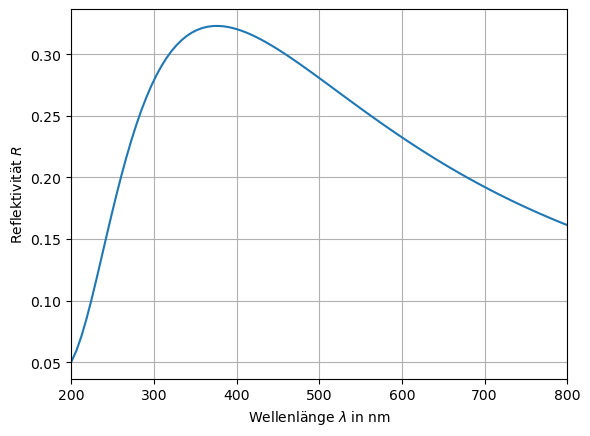
\includegraphics[width=0.7\textwidth]{1.png}
    \caption{Resultierender Plot}
\end{figure}

\end{document}